\documentclass[10pt,a4j,twocolumn]{jsarticle}
\usepackage[dvipdfmx]{graphicx}
%\usepackage[dvipdfmx]{hyperref}
\usepackage{url}
\usepackage{here}

\setlength{\textheight}{275mm}
\headheight 5mm
\topmargin -30mm
\textwidth 185mm
\oddsidemargin -15mm
\evensidemargin -15mm
\pagestyle{empty}

\begin{document}
\title{Githubを利用したRuby初心者学習ソフトの開発}
\author{関西学院大学 情報科学科 西谷研究室 2549 浦田 航貴}
\date{}
\maketitle
\section{序論}
西谷研究室に在籍している学生は,Rubyプログラミングを修得するために初心者向けの問題集を使って学習している.\\
%「初学者がこれらのスキルを自然と身につけることはできないか?」という問いに対する一つの答えとしてruby\_noviceを開発する.
ruby\_noviceが目指すのは,学習者自身が出力チェックできるようにしRubyプログラミングにおけるテスト実行に自然と慣れるような学習形態である.さらに,進捗状況の管理や指導者からの添削をより容易におこなえるように改善するため,バージョン管理ソフトGithubを利用するシステムを開発した.本研究は,Ruby初心者が文法だけでなく,プログラミングにおける振舞いを身につけるための支援ソフトを開発することを目的としている.

\section{研究手法}
ruby\_noviceでは,学習者自身で書いたコードを開発現場で使用されている一般的なテスト環境でテストする.本研究でモデルとしたテスト駆動開発ならびに比較検討したフレームワークを下記に示す.
\subsection{TDD(Test Driven Development)}
プログラミング開発の最先端の技法としてTDDが奨励されている.TDDでは,仕様を満たすテストを書く(Red), テストと通るコードを書く(Green), コードを読みやすく直す(Refactoring)というステップでRubyプログラミングを進めていくことを基本としている.それぞれの段階で次に作業する目標が明確になり,コード開発の効率が上がる.
\subsection{test::unit}
Ruby用のxUnit 系の単体テストフレームワークである.Ruby1.8までは Ruby本体に標準添付されていたが,Ruby1.9.1からはminitestというフレームワークが標準添付されている\cite{1}.
\subsection{aruba}
arubaは,Cucumber,RSpec,Minitestのような人気のあるTDD/BDD フレームワーク
でコマンドラインアプリケーションのテストを簡単で楽しいものにする拡張である\cite{2}.
\section{開発ソフトの仕様}
本研究で開発したソフトruby\_noviceは,以下の3つの機能を有している.
\begin{enumerate}
\item  Rubyの標準ライブラリ配布機構であるrubygemsに従っている
\item Githubを使って生徒のレポート提出機構を提供している
\item arubaにより生徒自身によるテスト機能を提供している
\end{enumerate}

%各章の概要は,以下の通りである.\\
%*第1章 (list1.1 〜 1.7):  putsメソッドやpメソッド\\
%*第3章 (list3.1 〜 3.11): ファイルの読み込み\\
%*第4章 (list4.1):        ローカル変数とグローバル変数\\
%*第5章 (list5.1 〜 5.5):  条件判断(if, unlessなど)\\
%*第6章 (list6.1 〜 6.13): 繰り返し(for,times,whileなど)\\
%*第7章 (list7.1 〜 7.4):  メソッド\\

ruby\_novice の構造は,図1のように3つに分かれている.
\begin{figure}[H]
\begin{center}
     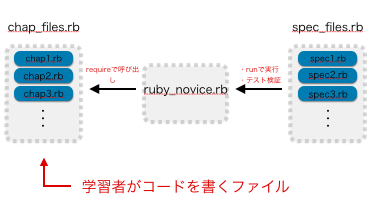
\includegraphics[width=9cm, bb=0 0 644 342]{abst.jpg}
     \caption{ruby\_noviceの構造.}
\end{center}
%\vspase{0\baselineskip}
\end{figure}

\begin{itemize}

\item chap\_files.rb (chap1.rb ...) : Textのコードを書く部分.

\item ruby\_novice.rb : chap\_files.rbを呼び出している.

\item spec\_files.rb : 出力結果 = 期待している値の検証.

\end{itemize}

現状は,「たのしいRuby」の第1章〜第7章までのテストを実装できる.テスト環境としては,環境変数RUBYNOVICE\_NAMEにディレクトリ名を入れるだけで,個人ごとにテストすることができる.また各章ごとや各問題ごとにテストができ,1問ずつ確認しながらコードを書いていくことが可能である.

\section{考察}
arubaは, print をそのまま出力でき,テストが可能である学習者がtextを見ながら書いていけるというメリットがあるので学習コストや間違えるリスクを削減できる.

今後の課題としては,現段階でtextの7章までしかテストコードを書けていないので引き続き書くことである.また問題にClassがあるコード(8章)は, 今まで通りコードを写すだけではテストできないので別のTDDフレームワークと比較して考える必要がある.


\begin{flushleft}
\begin{thebibliography}{9}

\bibitem{1}「test-unit - Ruby用単体テストフレームワーク」伊藤淳一, \url{https://test-unit.github.io/ja/}, 2017/2/12アクセス.
\bibitem{2}「Qiita Aruba gemでCLIのテストを支援する」, tbpgrさん, \url{http://qiita.com/tbpgr/items/41730edcdb07bb5b59ad}, 2017/2/12アクセス.

\end{thebibliography}
\end{flushleft}



\end{document}